\chapter{Analysis of the application state}

In this chapter, I will introduce a web application helping with teaching database systems subject at the university. \\
I will describe the current and planned state of the application from the perspective of application architecture, design patterns, and used technology stack. The goal is to identify the existing problems of the current application, outline how some of them will be solved in a new portal, as well as indicate what difficulties we can face developing the new application using a new stack of technologies and new architecture.

\section{The BI-DBS portal}
The BI-DBS portal is a web application used for teaching database systems subject in a bachelor's study program at the Czech Technical University at the Faculty of Information Technology. The portal is complex and has many useful functionalities. It allows managing and tracking all the student's studying progress during the semester, including semester tests, complex semester work, and exams. Besides teachers have an overview of all their student's work in one place.
The current application was developed as well as a new one being developed by students and teachers in subjects BI-SP1, BI-SP2 subjects, and theses. That is a unique fact about this project. Every half or one year new students get to the application development. They are open to sharing their ideas for improving the application, thus we are designing and implementing a better and better product each year.

%%%%%%%%%%%%%%%%%%%%%%%%%%%%%%%%%%%%%%%%%%%%%%%%%%%%%%%%%%%%%%%%

\section{Current state of the application}
The current BI-DBS portal was deployed for the first time in 2016. Over time it gained new features and grew large. Used technologies became not relevant and it became difficult to maintain it. 

\subsection{Architecture}
The current application was built in a traditional way, using a monolithic architecture approach and following the Model-View-Presenter architectural pattern\cite{potel_mvp}. Figure 1.1 shows the visualization of the acritecture. The application is presented as one monolithic unit, and it is composed  of three components.

\begin{itemize}
  \item The model: Communicates with the database and handles domain and business logic.
  \item The view: Provides visualization and directs user commands to the presenter, does not contain logic.
  \item The presenter: Manages interactions between the database and the view. Receives data from the model and formats it to display in the view.
\end{itemize}

\begin{figure}[hp]
\centering
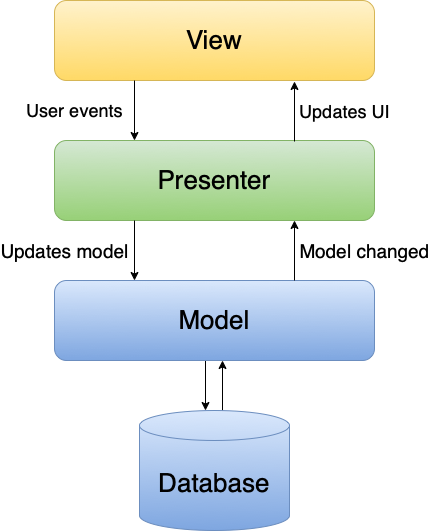
\includegraphics[scale=0.5]{../png/mvp_monolithic.png}
\caption{Monolithic architecture, MVP pattern}\label{picture:mvp}
\end{figure}

\noindent
This architecture's main concept is having one code base that benefits in \\simplifying development, testing, debugging, and deployment. \\
However, we can have those benefits only until the application grows large. Then all those processes get slower, more complex, and become problematic. In addition, with a lack of flexibility and scalability, it becomes challenging to maintain the application and keep it secure. \\

\noindent The BI-DBS portal is being developed by students. Students generally do not have much experience developing large applications and dealing with complex dependencies. Besides, they have limited time to progress in learning and developing the portal. Therefore it takes a lot of time for students to learn before contributing to the project. Thus it is more challenging to keep the application maintainable and ... (just one more example)

%%%%%%%%%%%%%%%%%%%%%%%%%%%%%%%%%%%%%%%%%%%%%%%%%%%%%%%%%%%%%%%%

\subsection{Technologies}
\paragraph*{PHP.} PHP is a general-purpose, open-source scripting language that can be integrated into HTML. It differs from client-side scripting languages in that its HTML is generated on a server and then sent to a client. That feature allows rapidly building a web application with a thick server and thin client. This is one of the approaches to using PHP to build an application, and it is used in the current project.

\paragraph*{Doctrine.} "Doctrine ORM is an object-relational mapper for PHP 7.1+ that provides transparent persistence for PHP objects. It sits on top of a powerful database abstraction layer. One of its key features is the option to write database queries in a proprietary object-oriented SQL dialect called Doctrine Query Language."


\paragraph*{Nette.} Nette is an open-source framework for creating web applications in PHP. It helps with developing both the client and server sides of the application. The disadvantage of it is the strong dependencies between frontend and backend. That makes it problematic to adjust something on one side without affecting another one.

\paragraph*{Latte.} Nette framework is using a template system Latte. It compiles templates down to the optimal PHP code. 

\paragraph*{AdminLTE.} AdminLTE is a fully responsive administration template. Based on Bootstrap 4.6 framework and also the JS/jQuery plugin. 

\paragraph*{Webpack.}"At its core, webpack is a static module bundler for modern JavaScript applications. When webpack processes your application, it internally builds a dependency graph from one or more entry points and then combines every module your project needs into one or more bundles, which are static assets to serve your content from."




% \subsection{Sources}
% Webpack - https://webpack.js.org/concepts/
% Doctrine - https://github.com/doctrine/orm
% Latte - https://latte.nette.org/en/
% Nette - https://nette.org/en/
% HTML - https://developer.mozilla.org/en-US/docs/Web/HTML
% php - https://www.php.net/manual/en/intro-whatis.php
% monolithic - https://www.atlassian.com/microservices/microservices-architecture/microservices-vs-monolith ,
% https://www.qulix.com/about/monolithic-vs-microservices-architechture/



\section{Planned state of the application}
% \subsection{Architecture}
% \subsection{Technologies}
